\chapter{Experiments}\label{ch:experiments}

Unless stated otherwise, numbers are medians over the three seeds, coefficient errors are relative Frobenius errors, and valid prediction times (VPT) are in Lyapunov times. Every number in this chapter is exported to \texttt{results/metrics/}.

\section{Data, conditioning and identifiability}\label{sec:exp-data}

\Cref{fig:attractors} shows the reference orbits and \cref{fig:corruption} the observation records at three corruption levels. At $\dto=4\tc/15$ an experiment contains only 25 samples, about four per oscillation. The peaks of the signal are no longer resolved, and an observer would struggle to draw the trajectory between consecutive points.

\begin{figure}[t]
  \centering
  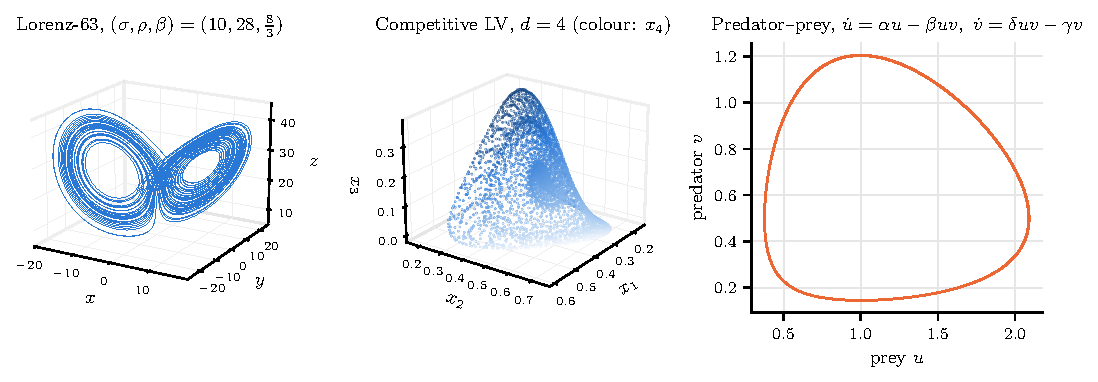
\includegraphics[width=\textwidth]{fig01_attractors}
  \caption{Reference attractors. Left: Lorenz-63. Centre: the four-species competitive Lotka--Volterra model, projected on $(x_1,x_2,x_3)$ and coloured by $x_4$. Right: the periodic predator--prey control.}
  \label{fig:attractors}
\end{figure}

\begin{figure}[t]
  \centering
  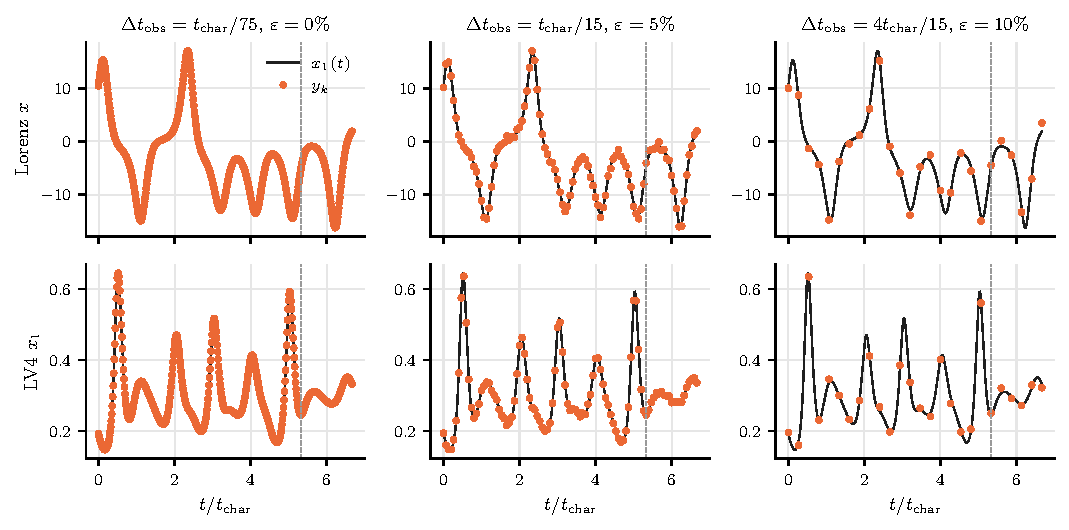
\includegraphics[width=\textwidth]{fig01_corruption}
  \caption{First experiment of a training record at three corruption levels (seed 0). The dashed line separates the fitting block from the held-out block.}
  \label{fig:corruption}
\end{figure}

\Cref{fig:spectrum} reports the singular values of the normalised library matrix $\Th(Z)/\sqrt N$ on noise-free data. For Lorenz-63, $\sigma_{\min}\approx0.025$ and the condition number is about $120$, whether the record is one orbit or four perturbed experiments. The competitive LV model is very different. On a single orbit $\sigma_{\min}=1.6\times10^{-5}$ ($\kappa=2.3\times10^{5}$); four experiments raise it to $1.3\times10^{-4}$ ($\kappa=3.4\times10^{4}$), an eight-fold improvement that is still two orders of magnitude worse than Lorenz. By \eqref{eq:ident}, a derivative error of $1\%$ of the signal can then produce coefficient errors of order one. This is what we observe: on noise-free data the Savitzky--Golay and weak estimators recover the LV4 coefficients to $10^{-4}$ or better, but at $\varepsilon=1\%$ every classical estimator returns coefficient errors between $1.06$ and $1.63$ with either design (\cref{tab:design}). The four-species attractor is a thin, nearly two-dimensional object on which several quadratic monomials are almost collinear. Equation recovery from noisy single-regime data is ill-posed there for any estimator, and the experiments below confirm that no method escapes this limit, although some forecast well despite it.

\begin{figure}[t]
  \centering
  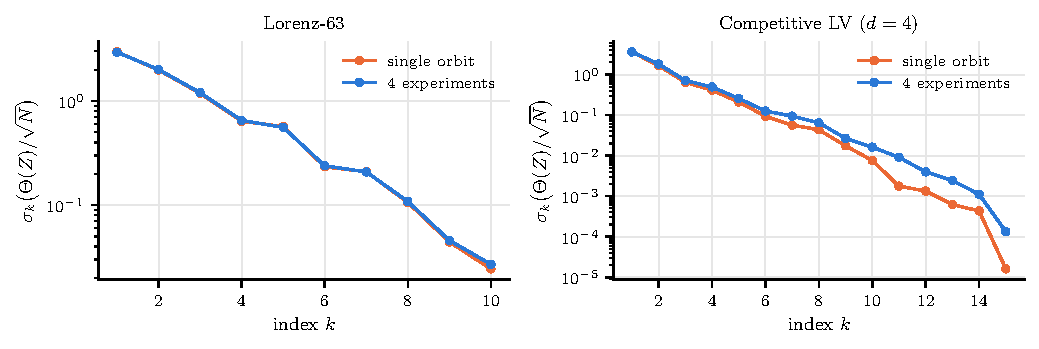
\includegraphics[width=0.9\textwidth]{fig01_library_spectrum}
  \caption{Singular values of the normalised library matrix on noise-free records of equal length, averaged over 5 seeds. Four short perturbed experiments help LV4 by about one order of magnitude in $\sigma_{\min}$, while Lorenz is already well conditioned.}
  \label{fig:spectrum}
\end{figure}

\begin{table}[t]
\centering
\caption{Design ablation at $\dto=\tc/75$: median coefficient error for a single orbit versus four perturbed experiments of the same total length.}
\label{tab:design}
\small
\begin{tabular}{llccccc}
\toprule
system & design & $\varepsilon$ & C1 & C2-FD & C2-SG & C3 \\
\midrule
\multirow{4}{*}{Lorenz} & single orbit & 0\% & 0.018 & 0.0063 & $1.0{\times}10^{-4}$ & $<10^{-6}$ \\
 & 4 experiments & 0\% & 0.013 & 0.0059 & $1.0{\times}10^{-4}$ & $<10^{-6}$ \\
 & single orbit & 1\% & 0.033 & 0.0090 & 0.0075 & 0.0031 \\
 & 4 experiments & 1\% & 0.039 & 0.0067 & 0.0050 & 0.0004 \\
\midrule
\multirow{4}{*}{LV4} & single orbit & 0\% & 0.31 & 0.15 & $1.0{\times}10^{-4}$ & $<10^{-6}$ \\
 & 4 experiments & 0\% & 0.18 & 0.0052 & $4.0{\times}10^{-4}$ & $<10^{-6}$ \\
 & single orbit & 1\% & 3.02 & 2.33 & 3.17 & 2.24 \\
 & 4 experiments & 1\% & 1.63 & 1.56 & 1.06 & 1.53 \\
\bottomrule
\end{tabular}
\end{table}

\section{Classical estimators on the full grid}\label{sec:exp-classical}

\Cref{fig:classical} summarises the classical fits (678 on the main grid, the irregular-sampling condition and the control). On Lorenz-63 the ranking is stable. Weak SINDy is best wherever anything works. Its error at $\varepsilon=1\%$ grows from $4\times10^{-4}$ at $\dto=\tc/75$ to $0.006$ at $\tc/15$ and $0.23$ at $2\tc/15$, and the method fails at $4\tc/15$ ($2.4$). The derivative-based estimators degrade one sampling step earlier. Savitzky--Golay SINDy has error $0.005$ at $\tc/75$, $0.16$ at $\tc/15$ and $1.7$ at $2\tc/15$, close to the $2.9\%$ and $11.7\%$ derivative biases predicted by \eqref{eq:fd}. At the coarsest interval, the estimators that do not diverge collapse onto fixed points or limit cycles: the Benettin exponent of their free runs drops to zero, and $W_1$ rises above one standard deviation. Dense least squares is never competitive.

Two further observations bear on the neural results. First, the weak form is sensitive to the \emph{distribution} of sampling times. With random sampling at the same mean density as $\tc/15$, the largest gaps exceed five times the mean interval, and weak SINDy fails even on noise-free data, whereas finite differences on the non-uniform grid lose accuracy more gracefully (\texttt{classical\_grid.csv}, irregular rows). Second, the failure at coarse sampling is not specific to chaos. On the periodic predator--prey control, every classical estimator has a coefficient error above $0.7$ for $\dto\ge2\tc/15$, including on noise-free data. The limit comes from resolving the signal, not from predictability.

\begin{figure}[t]
  \centering
  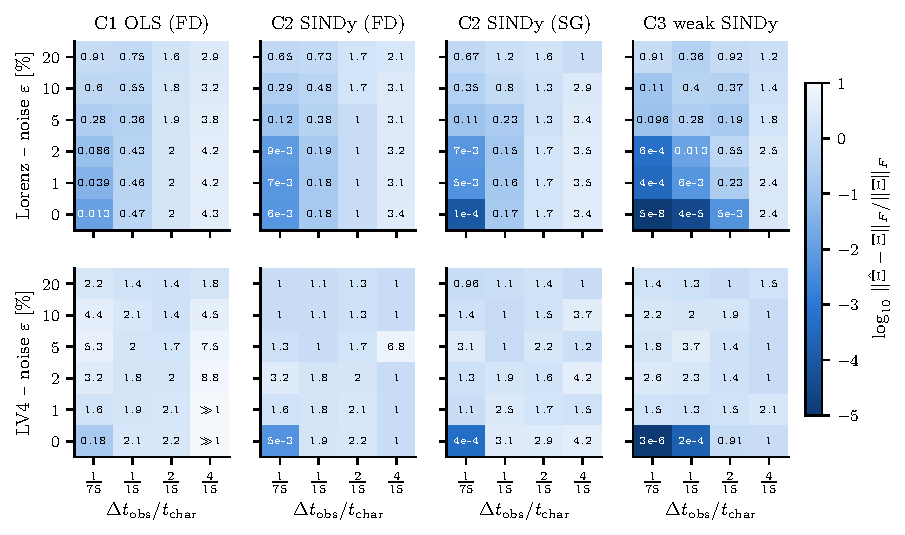
\includegraphics[width=\textwidth]{fig02_classical_heatmaps}
  \caption{Classical estimators: median relative coefficient error over the full sampling $\times$ noise grid (three seeds per cell). Darker is better.}
  \label{fig:classical}
\end{figure}

\section{Benchmark: neural versus classical identification}\label{sec:exp-bench}

\Cref{fig:bench-coef,fig:vpt} and \cref{tab:lorenz,tab:lv4} compare all seven estimators on the cross-shaped sub-grid.

\paragraph{Equation recovery at coarse sampling.} The clearest result concerns the sparse-library model N2 on Lorenz-63 at $\varepsilon=1\%$. Its median coefficient error is $0.009$ at $\dto=\tc/15$, against $0.006$ for weak SINDy. At $2\tc/15$ it is $0.031$, eight times lower than weak SINDy ($0.23$). At $4\tc/15$, where every classical estimator fails ($\ge2.4$), it is $0.052$. On noise-free data at $\tc/15$, N2 recovers the exact support for all seeds with error $<10^{-4}$. For LV4 the same holds without noise (error $10^{-3}$, exact support). Free runs of the N2 models reproduce the invariant statistics as well as the exact equations do: $W_1=0.08$ at $4\tc/15$, compared with $0.08$ for the exact vector field run for the same duration, and an estimated $\lmax=0.93$.

\paragraph{Noise.} At $\dto=\tc/15$ the advantage of N2 shrinks as noise grows. At $2\%$, weak SINDy is slightly better ($0.013$ versus $0.021$). At $5\%$ and $10\%$, N2 is better ($0.09$ versus $0.28$, and $0.21$ versus $0.40$). At $20\%$ no estimator is below a coefficient error of $0.36$. Multiple shooting with latent states performs the denoising, and the integral of the model replaces the integral of the noisy data. Neither helps once the noise standard deviation is comparable to the change of the state over a window.

\paragraph{Black-box model.} The distilled equations of N1 are never competitive. Their errors are between $0.21$ and $1.15$ on Lorenz and above $1.5$ on LV4, with dense supports. As a forecaster, N1 is better than the derivative-based estimators at coarse sampling (VPT $1.1$ versus $\le0.17$ at $4\tc/15$) but worse than the sparse models at fine sampling (VPT $1.2$--$1.8$ against $2.9$--$9.1$ for weak SINDy and N2). Its out-of-distribution VPT is $0.015$ Lyapunov times in every configuration: started off the attractor, the network leaves the observed region of state space immediately and its predictions are meaningless from the first step. Sparse library models with the right support extrapolate correctly by construction. N2 keeps an OOD VPT of $3.3$--$7.1$ on Lorenz at $1\%$ noise across all sampling intervals.

\paragraph{LV4: forecasting despite non-identifiability.} On LV4 at $\varepsilon=1\%$ no estimator recovers the coefficients. Even so, N2 has the longest VPT at every sampling interval: $3.4$ Lyapunov times at $\tc/15$, against $1.4$ for the best classical estimator, and $1.7$ at $4\tc/15$, against $0.16$. Its OOD VPT is $0.65$ against at most $0.06$. Its coefficients are wrong in directions that the attractor does not excite (\cref{sec:exp-data}). Trajectory matching selects among the many equivalent models one that is dynamically consistent with the data, whereas derivative regression amplifies noise along exactly those directions.

\paragraph{Warm starts.} N2-WS, which adds the weak-SINDy estimate to the initialisations, selected that initialisation in 22 of 54 fits, yet its results match N2 to within seed-to-seed variation everywhere. Once the flow-map stage and the continuation are in place, the final model depends little on which of the reasonable starting points is used. This is consistent with the basin study in \cref{sec:exp-landscape}.

\begin{figure}[t]
  \centering
  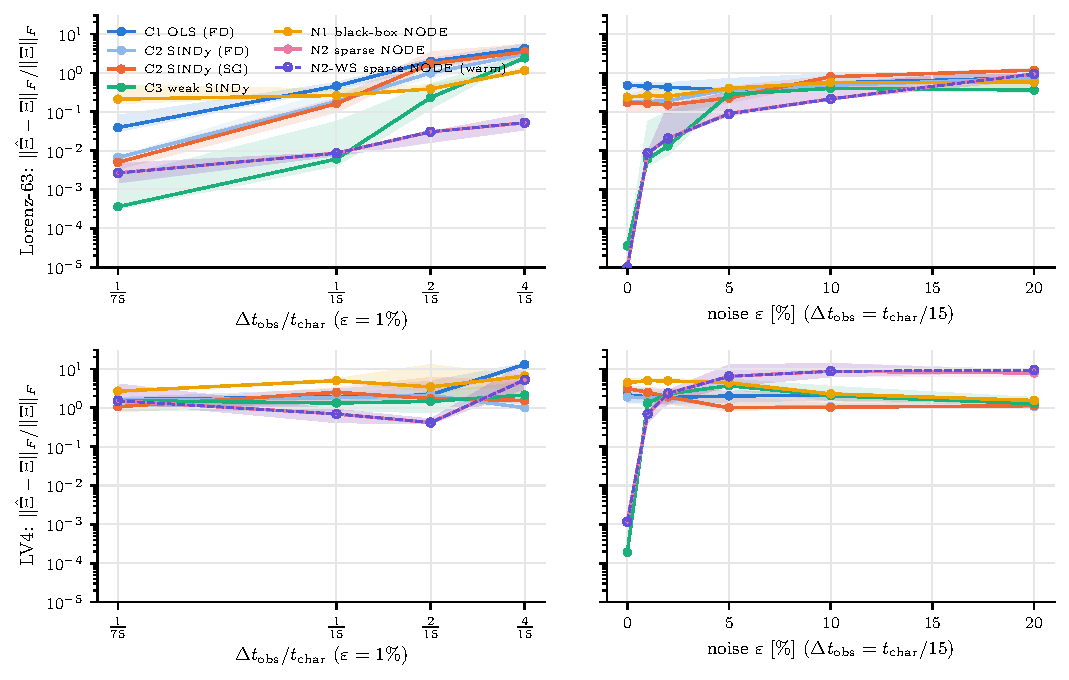
\includegraphics[width=\textwidth]{fig06_benchmark_coef}
  \caption{Coefficient error on the cross-shaped sub-grid: sampling sweep at $\varepsilon=1\%$ (left) and noise sweep at $\dto=\tc/15$ (right). Lines show medians and bands the inter-quartile range over seeds. The N1 curve is for its distilled equations.}
  \label{fig:bench-coef}
\end{figure}

\begin{figure}[t]
  \centering
  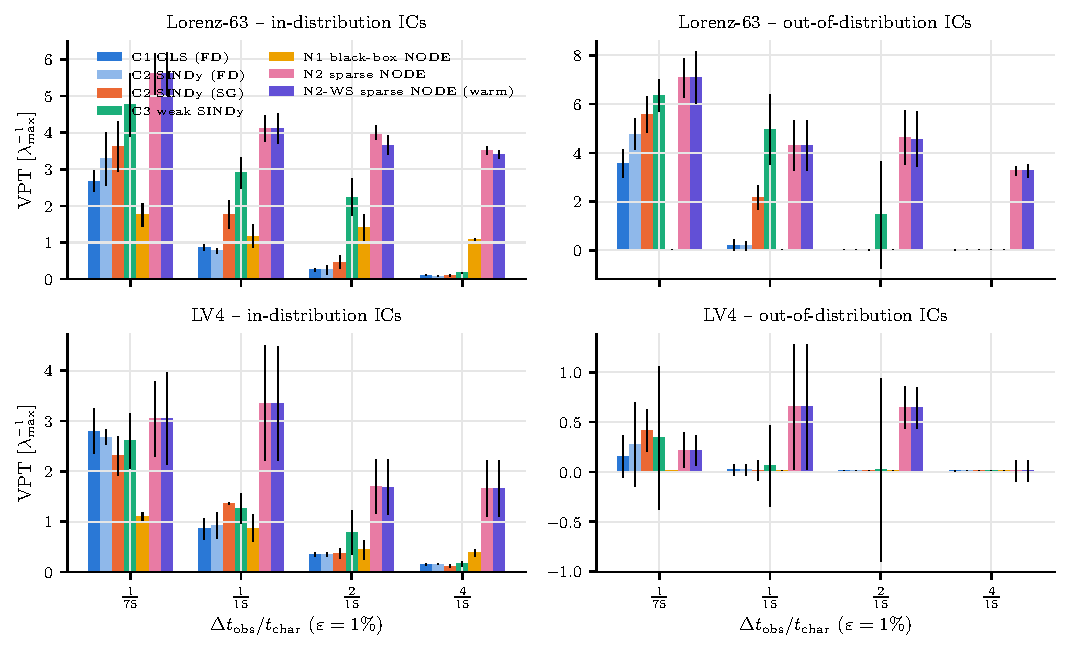
\includegraphics[width=\textwidth]{fig06_vpt}
  \caption{Valid prediction time at $\varepsilon=1\%$ from 16 in-distribution (left) and 16 out-of-distribution (right) initial conditions. Bars show medians over seeds, whiskers the standard deviation. For reference, the exact vector field reaches $11.3$ (Lorenz) and $8.1$ (LV4) in-distribution with the same integrator.}
  \label{fig:vpt}
\end{figure}

\begin{table}[t]
\centering
\caption{Lorenz-63: medians over three seeds in three regimes: \emph{moderate} ($\dto=\tc/15$, $\varepsilon=1\%$), \emph{sparse} ($\dto=4\tc/15$, $\varepsilon=1\%$) and \emph{noisy} ($\dto=\tc/15$, $\varepsilon=10\%$). VPT is in Lyapunov times, $W_1$ in standard deviations; ``--'' marks a divergent free run. $^\dagger$Equation metrics of N1 refer to its distilled equations, forecast metrics to the network.}
\label{tab:lorenz}
\resizebox{\textwidth}{!}{%
\begin{tabular}{l*{15}{c}}
\toprule
 & \multicolumn{5}{c}{moderate} & \multicolumn{5}{c}{sparse} & \multicolumn{5}{c}{noisy} \\
\midrule
 & coef. err. & $F_1$ & VPT$_{\rm ID}$ & VPT$_{\rm OOD}$ & $W_1$ & coef. err. & $F_1$ & VPT$_{\rm ID}$ & VPT$_{\rm OOD}$ & $W_1$ & coef. err. & $F_1$ & VPT$_{\rm ID}$ & VPT$_{\rm OOD}$ & $W_1$ \\
\midrule
C1 OLS (FD) & 0.46 & 0.38 & 0.86 & 0.22 & 0.08 & 4.25 & 0.38 & 0.11 & 0.01 & -- & 0.55 & 0.38 & 0.59 & 0.13 & 0.05 \\
C2 SINDy (FD) & 0.18 & 0.67 & 0.77 & 0.18 & 0.16 & 3.09 & 0.38 & 0.09 & 0.01 & 1.53 & 0.48 & 0.80 & 0.67 & 0.16 & 0.08 \\
C2 SINDy (SG) & 0.16 & 0.64 & 1.77 & 2.18 & 0.11 & 3.47 & 0.39 & 0.09 & 0.01 & 1.53 & 0.80 & 0.48 & 0.68 & 0.14 & 0.11 \\
C3 weak SINDy & 6.1e-3 & 1.00 & 2.90 & 4.96 & 0.14 & 2.43 & 0.46 & 0.17 & 0.01 & 1.11 & 0.40 & 0.48 & 1.66 & 0.06 & 0.14 \\
N1 black-box NODE$^\dagger$ & 0.26 & 0.82 & 1.17 & 0.02 & 0.22 & 1.15 & 0.45 & 1.08 & 0.02 & 0.17 & 0.57 & 0.52 & 1.38 & 0.02 & 0.30 \\
N2 sparse NODE & 8.6e-3 & 1.00 & 4.11 & 4.30 & 0.11 & 0.05 & 0.64 & 3.51 & 3.26 & 0.08 & 0.21 & 0.56 & 1.88 & 0.55 & 0.12 \\
N2-WS (warm start) & 8.6e-3 & 1.00 & 4.11 & 4.30 & 0.17 & 0.05 & 0.64 & 3.40 & 3.26 & 0.08 & 0.21 & 0.56 & 2.03 & 0.99 & 0.05 \\
\bottomrule
\end{tabular}}
\end{table}

\begin{table}[t]
\centering
\caption{Competitive LV ($d=4$), same regimes and conventions as \cref{tab:lorenz}.}
\label{tab:lv4}
\resizebox{\textwidth}{!}{%
\begin{tabular}{l*{15}{c}}
\toprule
 & \multicolumn{5}{c}{moderate} & \multicolumn{5}{c}{sparse} & \multicolumn{5}{c}{noisy} \\
\midrule
 & coef. err. & $F_1$ & VPT$_{\rm ID}$ & VPT$_{\rm OOD}$ & $W_1$ & coef. err. & $F_1$ & VPT$_{\rm ID}$ & VPT$_{\rm OOD}$ & $W_1$ & coef. err. & $F_1$ & VPT$_{\rm ID}$ & VPT$_{\rm OOD}$ & $W_1$ \\
\midrule
C1 OLS (FD) & 1.91 & 0.44 & 0.86 & 0.02 & 0.07 & 13.00 & 0.44 & 0.16 & 0.01 & 0.28 & 2.11 & 0.44 & 0.62 & 0.01 & 0.18 \\
C2 SINDy (FD) & 1.80 & 0.43 & 0.92 & 0.02 & 0.16 & 1.00 & 0.00 & 0.16 & 0.01 & 0.80 & 1.07 & 0.32 & 0.42 & 0.01 & 0.48 \\
C2 SINDy (SG) & 2.51 & 0.43 & 1.36 & 0.01 & 0.24 & 1.54 & 0.00 & 0.12 & 0.01 & 35.94 & 1.03 & 0.40 & 0.58 & 0.01 & 0.80 \\
C3 weak SINDy & 1.32 & 0.48 & 1.26 & 0.06 & 0.08 & 2.13 & 0.21 & 0.16 & 0.01 & 0.80 & 2.04 & 0.42 & 0.29 & 0.01 & 1.18 \\
N1 black-box NODE$^\dagger$ & 4.98 & 0.45 & 0.87 & 0.01 & 0.22 & 6.56 & 0.45 & 0.38 & 0.01 & 0.50 & 2.27 & 0.44 & 0.76 & 0.01 & 0.25 \\
N2 sparse NODE & 0.69 & 0.45 & 3.36 & 0.65 & 0.03 & 5.24 & 0.44 & 1.67 & 0.01 & 0.12 & 8.70 & 0.44 & 0.96 & 0.01 & 0.11 \\
N2-WS (warm start) & 0.69 & 0.45 & 3.36 & 0.65 & 0.03 & 5.24 & 0.44 & 1.67 & 0.01 & 0.12 & 8.70 & 0.44 & 0.96 & 0.01 & 0.11 \\
\bottomrule
\end{tabular}}
\end{table}


\begin{figure}[p]
  \centering
  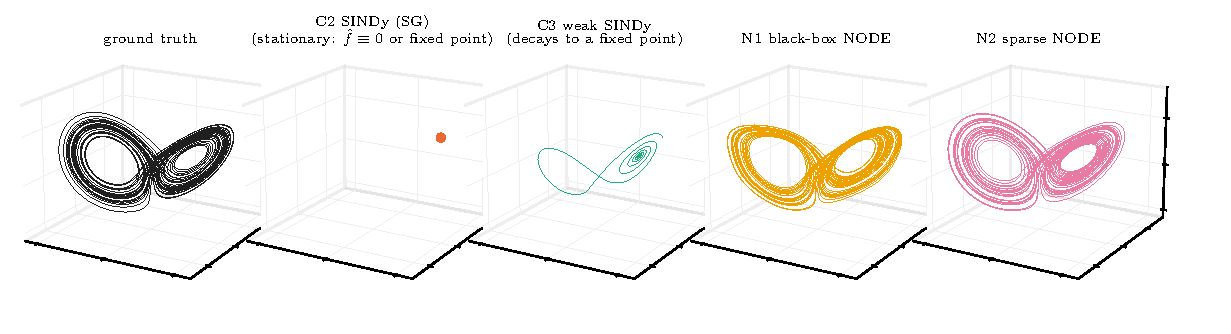
\includegraphics[width=\textwidth]{fig06_gallery_lorenz_dt0.267_n0.01}\\[2pt]
  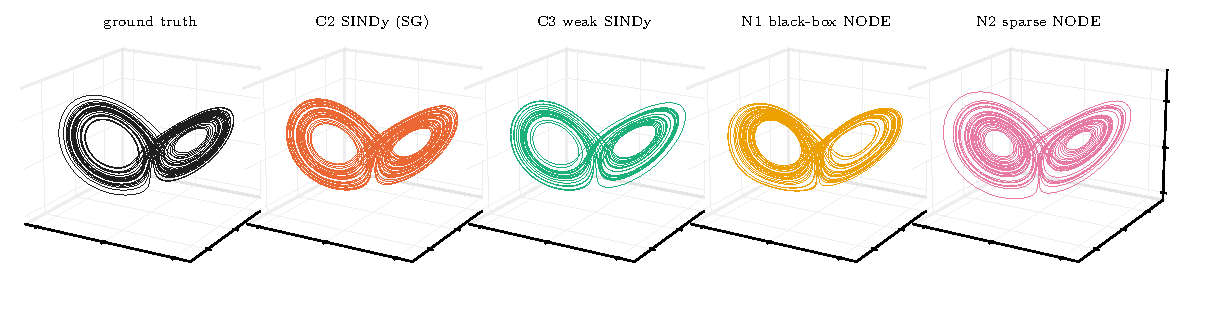
\includegraphics[width=\textwidth]{fig06_gallery_lorenz_dt0.067_n0.05}\\[2pt]
  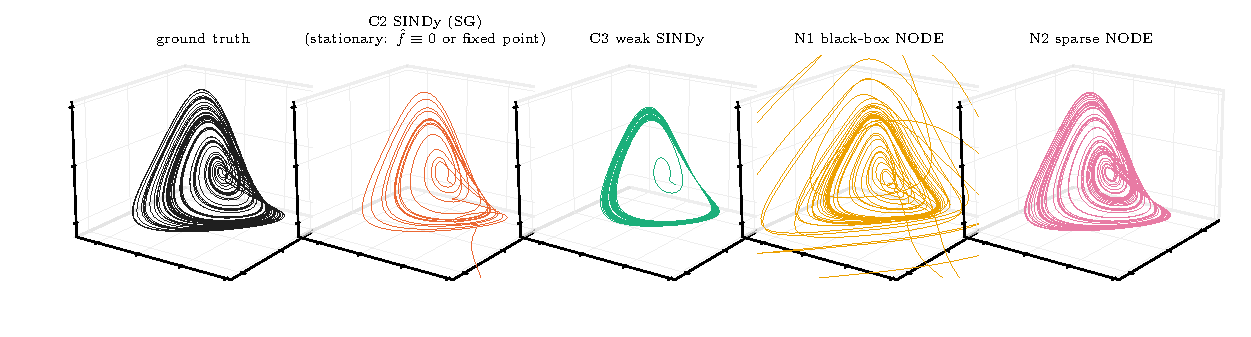
\includegraphics[width=\textwidth]{fig06_gallery_lv4_dt0.067_n0.01}
  \caption{Free runs over $60\tc$ of the identified models (seed 0). Top: Lorenz, $\dto=0.2$, $\varepsilon=1\%$. Middle: Lorenz, $\dto=0.05$, $\varepsilon=5\%$. Bottom: LV4, $\dto=\tc/15$, $\varepsilon=1\%$.}
  \label{fig:gallery}
\end{figure}

\section{Loss landscapes and nonconvex optimisation}\label{sec:exp-landscape}

\paragraph{Exact slices.} \Cref{fig:landscape} shows the trajectory-matching loss of Lorenz-63 as a function of $(\sigma,\rho)$, with $\beta$ at its true value and noise-free data. At $T=0.5$ ($0.45$ Lyapunov times) the single-shooting loss is a smooth valley around the truth. At $T=2$ the valley has narrowed into a curved ridge-bounded channel, and away from it the surface is flat at the level of the attractor's variance. At $T=8$ it is a ``golf course'': almost every parameter value gives the same, maximal loss, and the minimum occupies a thin filament of the grid. The one-dimensional slice in \cref{fig:landscape-slice} makes this precise. For $T=1$ the loss is a smooth funnel. For $T=4$ and $T=8$ it is flat, at the level of the attractor's variance, everywhere except in a dip around $\rho=28$ whose width is a small fraction of a unit. Away from the dip the curve carries irregular small-scale fluctuations: the gradient there is uninformative about the direction of the minimum. The multiple-shooting loss over the same record, with windows of $\tau=0.2$ restarted at the observations, decreases monotonically towards the truth over the whole interval and spans ten decades.

\begin{figure}[t]
  \centering
  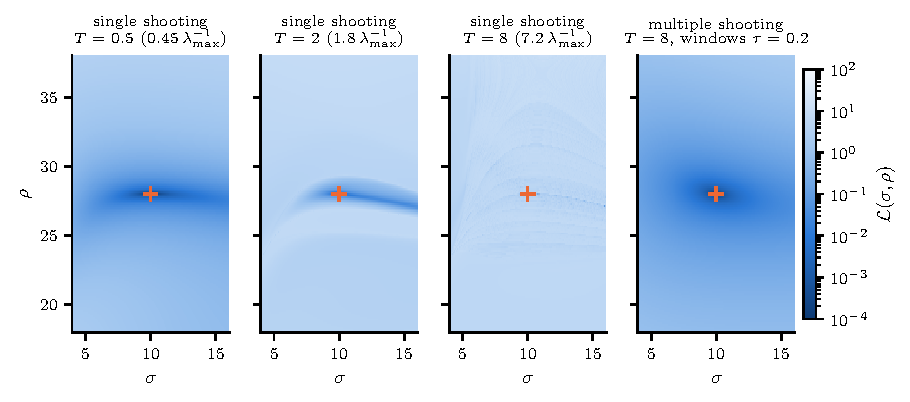
\includegraphics[width=\textwidth]{fig04_landscape_sigma_rho}
  \caption{Trajectory-matching loss $\mathcal L(\sigma,\rho)$ for Lorenz-63 on a $161\times161$ grid, noise-free data, $\beta=8/3$. The cross marks the truth. Single shooting over longer horizons (left three panels) against multiple shooting with $\tau=0.2$ over the longest horizon (right).}
  \label{fig:landscape}
\end{figure}

\begin{figure}[t]
  \centering
  \begin{subfigure}[t]{0.49\textwidth}
    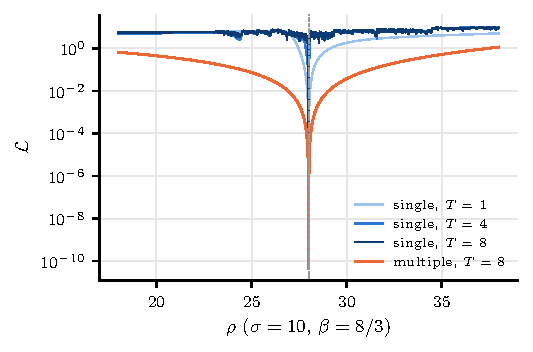
\includegraphics[width=\textwidth]{fig04_landscape_slice}
    \caption{Slice through the truth along $\rho$ (4\,001 points).}
    \label{fig:landscape-slice}
  \end{subfigure}\hfill
  \begin{subfigure}[t]{0.49\textwidth}
    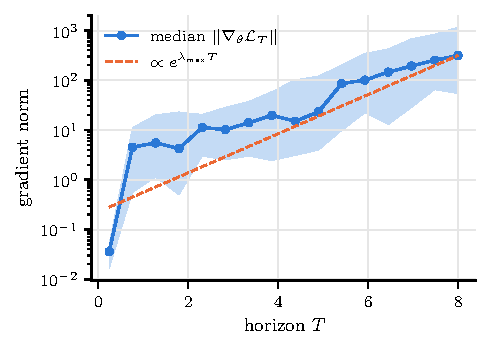
\includegraphics[width=\textwidth]{fig04_gradient_growth}
    \caption{Gradient norm against horizon at 64 points within $\pm5\%$ of the truth (median and 10--90\% band).}
    \label{fig:grad}
  \end{subfigure}
  \caption{Roughness and gradient growth of single shooting.}
\end{figure}

\paragraph{Gradient growth.} \Cref{fig:grad} confirms the mechanism of \cref{prop:basin}. Between $T=2$ and $T=8$ the median gradient norm grows exponentially at a fitted rate of $0.68$, against $\lmax=0.91$. The rate is lower than $\lmax$ for two reasons: the loss averages residuals over the horizon, so early, less sensitive residuals dilute the growth, and the residuals saturate at the size of the attractor once trajectories decorrelate. Over the horizon of $T=8$ the gradient norm still changes by four orders of magnitude, and the 10--90\% band spans more than an order of magnitude at every $T$. No single learning rate is appropriate across horizons, which is the practical side of the roughness.

\paragraph{Basins of attraction (three parameters).} \Cref{fig:basins-param} and \cref{tab:basins} report 96 random restarts of $(\sigma,\rho,\beta)$ estimation from a 1\%-noise record of length 4, using Adam on $\log\theta$.
\begin{itemize}
  \item \emph{Single shooting.} With $T=1$, $42\%$ of the starts reach the truth to within $1\%$. With $T=4$ none do, and only one start in 96 reaches $5\%$.
  \item \emph{Multiple shooting, short windows.} With windows of $K=4$ intervals ($0.2$ time units) and nodes at the observations, all 96 starts converge to the same point, $0.09\%$ from the truth.
  \item \emph{Multiple shooting, long windows.} With $K=20$ ($1$ time unit), all starts again converge to a single point, with or without a $K$-curriculum, but that point is $2.0\%$ from the truth. The noisy observations used as shooting nodes are amplified over the longer windows, and the minimiser itself is biased.
\end{itemize}
Long windows therefore cost accuracy when the nodes are fixed at noisy data. This is the errors-in-variables bias that the latent states $S$ in \eqref{eq:ms} remove.

\begin{table}[t]
\centering
\caption{Random restarts for $(\sigma,\rho,\beta)$: fraction of 96 starts within $1\%$ and $5\%$ of the truth, and median final error.}
\label{tab:basins}
\small
\begin{tabular}{lccc}
\toprule
objective & within 1\% & within 5\% & median error \\
\midrule
single shooting, $T=1$ & 0.42 & 0.42 & 0.34 \\
single shooting, $T=4$ & 0.00 & 0.01 & 0.16 \\
multiple shooting, $K=4$ ($\tau=0.2$) & 1.00 & 1.00 & $8.9\times10^{-4}$ \\
multiple shooting, $K=20$ ($\tau=1$) & 0.00 & 1.00 & 0.020 \\
multiple shooting, $K:1\to20$ & 0.00 & 1.00 & 0.020 \\
\bottomrule
\end{tabular}
\end{table}

\begin{figure}[t]
  \centering
  \begin{subfigure}[t]{0.44\textwidth}
    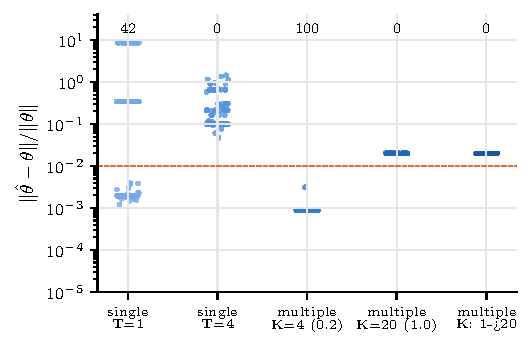
\includegraphics[width=\textwidth]{fig04_basins_parametric}
    \caption{Final relative error of 96 restarts for $(\sigma,\rho,\beta)$. Numbers at the top give the percentage of starts within $1\%$ of the truth (dashed line).}
    \label{fig:basins-param}
  \end{subfigure}\hfill
  \begin{subfigure}[t]{0.54\textwidth}
    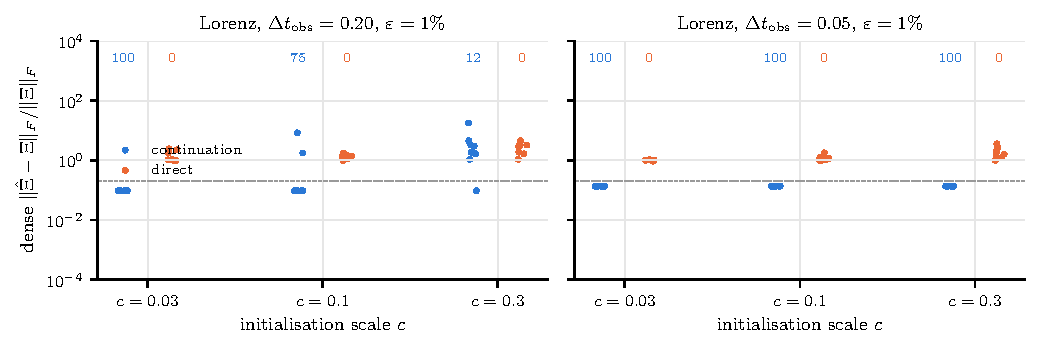
\includegraphics[width=\textwidth]{fig04_basins_library}
    \caption{Random restarts of the 30-coefficient library problem (8 per scale): continuation versus direct training at $K_{\max}$. Numbers at the top give the percentage of runs below the dashed line (dense error $0.2$).}
    \label{fig:basins-lib}
  \end{subfigure}
  \caption{Basins of attraction.}
\end{figure}

\paragraph{Basins of attraction (full library).} \Cref{fig:basins-lib} repeats the experiment for the 30-coefficient library problem with random initialisations $\tilde\Xib_0=c\,\mathcal N(0,\overline{\tilde\Xib_{\rm OLS}^2})$, which use no information about the truth. Training directly at the final window length fails for every start, at every scale and both sampling intervals: none of the 48 runs gets below a dense coefficient error of $0.2$, and most produce non-finite rollouts at the first iteration. With the continuation of \cref{alg:n2}, every start converges at $\dto=0.05$, for all three scales, to the same dense solution, with error $0.14$ before thresholding; after thresholding, the models of the main sweep reach $0.009$ in this configuration. At $\dto=0.2$ the continuation succeeds for $100\%$, $75\%$ and $12\%$ of the starts at $c=0.03$, $0.1$ and $0.3$. The flow-map stage must begin from a field whose one-step map over $\dto=0.2$ stays bounded, and large random quadratic fields do not. This explains why the zero field is the most reliable initialisation in \cref{alg:n2} (selected in 31 of 54 N2 fits), and why multistart over a few such candidates suffices.


\paragraph{The black-box loss surface.} \Cref{fig:nn-landscape} shows filter-normalised slices of the N1 loss around the trained weights. With $K=1$ the trained weights sit at the bottom of a smooth, nearly quadratic bowl ($\log_{10}\mathcal L$ from $-2.9$ at the centre to $-0.5$ at the edges). With $K=15$, the training window, the bowl is narrower and anisotropic and is surrounded by a plateau about three decades higher. With $K=60$ ($4\tc$, close to single shooting) the minimum disappears. The trained weights lie on a broad plateau at the level of the attractor's variance ($\log_{10}\mathcal L\approx 0$), bounded by a cliff where perturbed networks produce unstable trajectories. The long-window objective cannot distinguish the trained model from networks perturbed by half a filter norm. Its gradient carries no information about the short-term dynamics that the model has learned, which is the network analogue of \cref{fig:landscape}.

\begin{figure}[t]
  \centering
  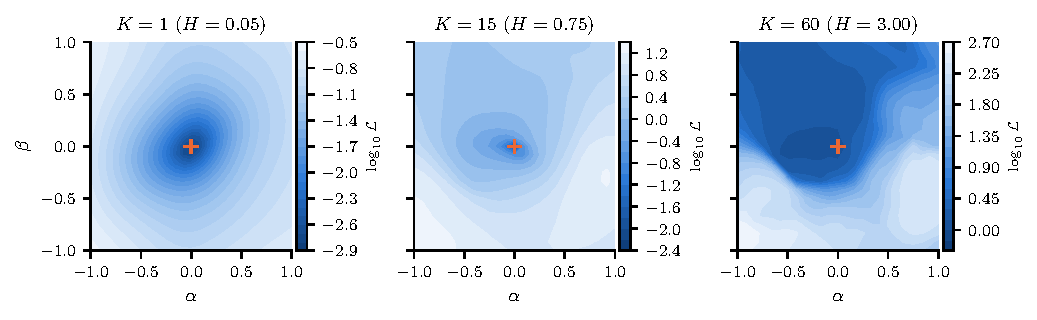
\includegraphics[width=\textwidth]{fig04_nn_landscape}
  \caption{Loss of the trained black-box model (Lorenz, $\dto=0.05$, $\varepsilon=1\%$) on two filter-normalised random directions, evaluated with windows of $K=1$, $15$ and $60$ observation intervals.}
  \label{fig:nn-landscape}
\end{figure}


\section{Uncertainty, stability and out-of-distribution generalisation}\label{sec:exp-uq}

\Cref{tab:uq} scores the four predictive distributions of \cref{sec:uq-theory} at $\dto=\tc/15$ and two noise levels. \Cref{fig:uq-bands} shows typical forecasts, and \cref{fig:uq-cal} the coverage and CRPS against lead time.

\begin{table}[t]
\centering
\caption{Predictive uncertainty at $\dto=\tc/15$, averaged over 16 initial conditions and the first 5 Lyapunov times. Coverage is that of central 90\% intervals (ideal: 0.90). CRPS is in units of $\sigma_i$ (lower is better). The spread--skill column is Spearman's $\rho$ between ensemble spread and the error of the ensemble mean. The shift ratio is the mean spread over the first Lyapunov time for OOD initial conditions divided by that for ID ones.}
\label{tab:uq}
\small
\begin{tabular}{llcccccccc}
\toprule
 & & \multicolumn{2}{c}{coverage} & \multicolumn{2}{c}{CRPS} & \multicolumn{2}{c}{spread--skill} & shift ratio \\
\cmidrule(lr){3-4}\cmidrule(lr){5-6}\cmidrule(lr){7-8}
system, $\varepsilon$ & method & ID & OOD & ID & OOD & ID & OOD & spread / error \\
\midrule
Lorenz, 1\% & E-SINDy (C3) & 0.87 & 0.93 & 0.16 & 0.22 & 0.89 & 0.81 & 15.4 / 20.9 \\
 & N2 bagging & 0.18 & 0.11 & 0.10 & 0.07 & 0.79 & 0.80 & 3.9 / 6.4 \\
 & N1 deep ens. & 0.41 & 0.47 & 0.51 & 1.35 & 0.61 & 0.13 & 11.9 / 23.5 \\
 & N1 MC dropout & 0.67 & 0.64 & 0.64 & 0.96 & 0.21 & -0.09 & 1.1 / 5.3 \\
\midrule
Lorenz, 10\% & E-SINDy (C3) & 0.75 & 0.76 & 0.42 & 0.78 & 0.58 & 0.34 & 11.2 / 10.7 \\
 & N2 bagging & 0.54 & 0.49 & 0.33 & 0.59 & 0.77 & 0.33 & 11.9 / 14.3 \\
 & N1 deep ens. & 0.40 & 0.47 & 0.50 & 0.99 & 0.62 & -0.12 & 9.8 / 17.8 \\
 & N1 MC dropout & 0.68 & 0.65 & 0.62 & 0.89 & 0.23 & -0.14 & 1.0 / 4.9 \\
\midrule
LV4, 1\% & E-SINDy (C3) & 0.95 & 0.95 & 0.57 & 3.31 & 0.68 & 0.53 & 110.1 / 25.6 \\
 & N2 bagging & 0.58 & 0.35 & 0.33 & 3.11 & 0.76 & 0.35 & 125.5 / 142.8 \\
 & N1 deep ens. & 0.38 & 0.47 & 0.65 & 2.65 & 0.25 & 0.10 & 7.4 / 6.8 \\
 & N1 MC dropout & 0.73 & 0.41 & 0.56 & 1.76 & 0.13 & 0.15 & 1.8 / 4.3 \\
\midrule
LV4, 10\% & E-SINDy (C3) & 0.85 & 0.83 & 6.90 & 8.49 & 0.56 & 0.24 & 1.2 / 1.2 \\
 & N2 bagging & 0.50 & 0.17 & 0.65 & 9.96 & 0.47 & 0.28 & 209.4 / 285.8 \\
 & N1 deep ens. & 0.36 & 0.50 & 0.66 & 2.46 & 0.26 & 0.04 & 7.2 / 6.5 \\
 & N1 MC dropout & 0.67 & 0.51 & 0.55 & 1.81 & 0.12 & 0.14 & 2.0 / 4.2 \\
\bottomrule
\end{tabular}
\end{table}

\paragraph{The bootstrap of the weak regression is the best calibrated.} On Lorenz at $1\%$ noise, E-SINDy intervals cover the truth $87\%$ (ID) and $93\%$ (OOD) of the time, against a nominal $90\%$. Their spread is strongly rank-correlated with the actual error ($\rho=0.89$ ID, $0.81$ OOD). The OOD spread is 15 times the ID spread, and the OOD error 21 times the ID error, so the ensemble flags the distribution shift almost in proportion. The calibration survives $10\%$ noise on Lorenz (coverage $0.75$). It breaks down for LV4 at $10\%$, where a few bootstrap members are unstable and inflate both the spread and the CRPS.

\paragraph{Window bagging gives the most accurate but an over-confident distribution.} N2 has the lowest CRPS in five of the eight comparisons; the exceptions are LV4 out of distribution and LV4 at $10\%$ noise in distribution, where the black-box ensembles are best. Its spread is informative (spread--skill $0.79$--$0.80$ on Lorenz at $1\%$) but far too small: the members are nearly identical, and coverage is only $0.18$ ID and $0.11$ OOD. Resampling windows perturbs a problem that the continuation solves almost deterministically, so the bootstrap explores a single basin. Its intervals need recalibration, for instance by inflating the spread on held-out data, before they can be read as probabilities.

\paragraph{Deep ensembles detect the shift; MC dropout does not.} For the black-box model, the deep ensemble's spread grows about tenfold out of distribution ($11.9\times$ on Lorenz at 1\%), which correctly signals that the forecasts should not be trusted. Its spread--skill correlation, however, drops from $0.61$ to $0.13$, and coverage stays below $0.5$. MC dropout with trajectory-wise masks produces a spread that is almost independent of the initial condition (ratio $1.0$--$2.0$), while its error grows four- to fivefold out of distribution. It also degrades the median forecast, which drifts away from the truth within one Lyapunov time even in distribution (\cref{fig:uq-bands}). In our setting dropout gives neither an accurate forecaster nor a useful detector of distribution shift.

\begin{figure}[t]
  \centering
  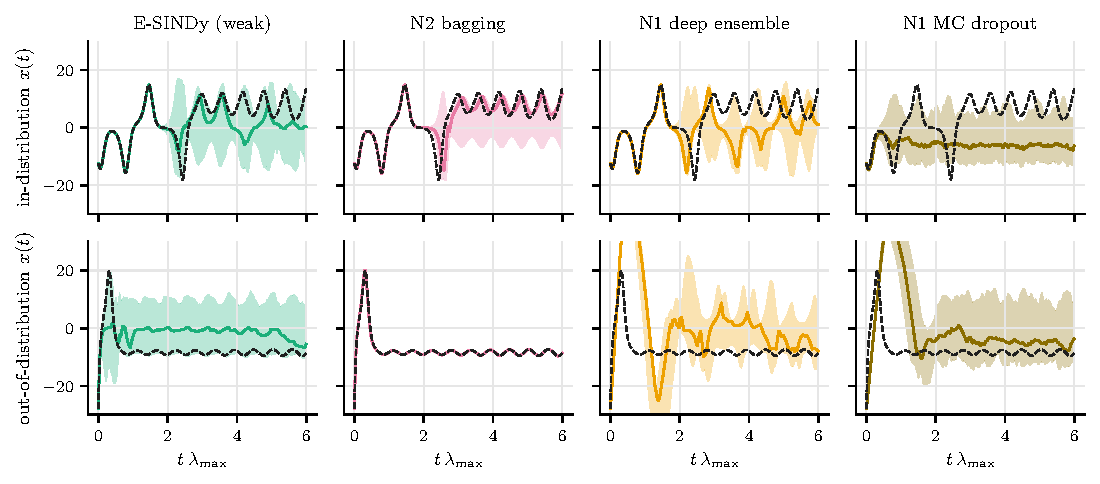
\includegraphics[width=\textwidth]{fig05_uq_bands}
  \caption{Forecasts of $x(t)$ for Lorenz ($\dto=0.05$, $\varepsilon=1\%$) from an in-distribution (top) and an out-of-distribution (bottom) initial condition. Lines show the median of the ensemble, bands the 5--95\% range, and the dashed line the truth.}
  \label{fig:uq-bands}
\end{figure}

\begin{figure}[t]
  \centering
  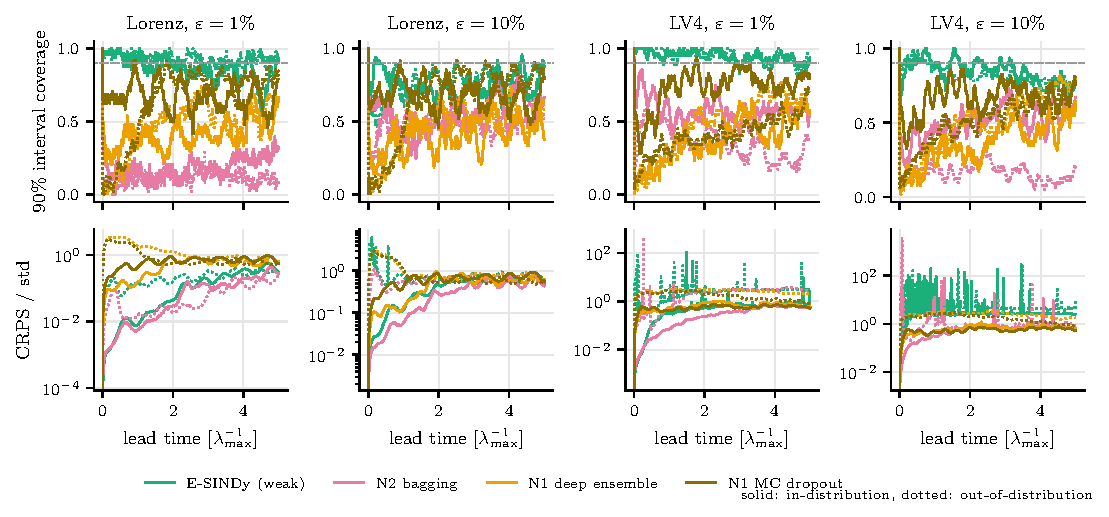
\includegraphics[width=\textwidth]{fig05_uq_calibration}
  \caption{Coverage of central 90\% intervals (top) and CRPS (bottom) against lead time, for in-distribution (solid) and out-of-distribution (dotted) initial conditions.}
  \label{fig:uq-cal}
\end{figure}

\paragraph{Uncertainty in the support.} \Cref{fig:inclusion} shows E-SINDy inclusion probabilities on Lorenz across noise levels. The true terms are kept in essentially every bootstrap sample up to $10\%$ noise. At $20\%$ the selected threshold rises and some true terms of the $\dot x$ and $\dot z$ equations are dropped in about half of the samples. The spurious terms behave differently in the three equations. The $\dot z$ equation stays clean up to $2\%$. In the $\dot x$ and $\dot y$ equations, spurious monomials appear in 10--25\% of the samples even without noise, in 30--60\% at $1$--$2\%$, and in almost all samples at $5$--$10\%$, although the point estimate has the exact support at low noise. The bootstrap is therefore more pessimistic than the point estimate. It locates the doubt in the equations where the library is nearly degenerate on the data: $x$ and $y$ are strongly correlated on the attractor, since $\dot x=\sigma(y-x)$ is small compared with $x$, and the constant, $z$ and $z^2$ columns are nearly collinear because $z$ stays far from zero.

\begin{figure}[t]
  \centering
  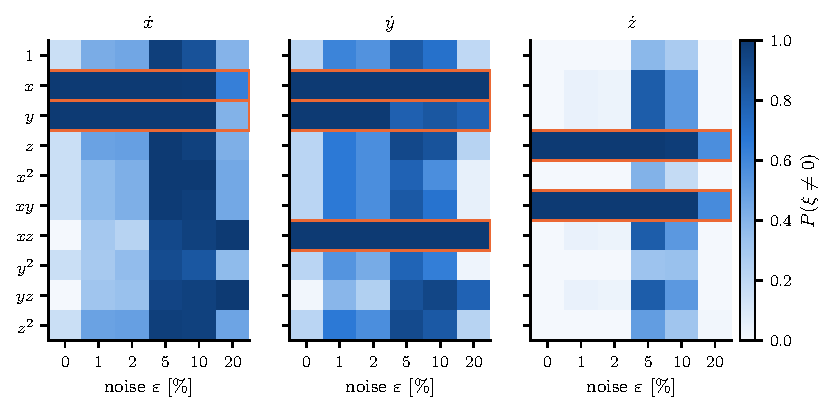
\includegraphics[width=\textwidth]{fig05_inclusion}
  \caption{E-SINDy inclusion probabilities $P(\xi_{kj}\neq0)$ for Lorenz at $\dto=0.05$ across noise levels (100 bootstrap samples). True terms are outlined.}
  \label{fig:inclusion}
\end{figure}


\section{Discussion}\label{sec:discussion}

\paragraph{When do neural models help?} The answer depends on what ``neural'' means. Integration through a differentiable solver brings a real gain over derivative-based and weak-form regression in one regime, coarse sampling at low noise. That gain is obtained by the sparse-library model, whose function class is the same as SINDy's. The black-box network adds nothing for equation discovery. It forecasts in-distribution only moderately, and it fails out of distribution without exception. The benefit therefore comes from the objective, matching trajectories instead of derivatives, and not from neural function approximation. Without the optimisation devices of \cref{sec:tm} this benefit is unreachable. Single shooting fails beyond about one Lyapunov time, and the flow-map stage needs a starting field whose one-step map is finite.

\paragraph{When does nothing help?} On the four-species LV model, coefficient recovery fails for every estimator as soon as the data are noisy. The singular values of the library show why: the attractor does not excite all directions of coefficient space, and four perturbed experiments improve $\sigma_{\min}$ by only an order of magnitude. The useful question is then not which estimator to use but which data to collect. Experiments that start further from the attractor, or interventions that drive the system through other regimes, would be needed. Short-term forecasts remain possible, and trajectory matching provides the best of them.

\paragraph{Limitations.}
\begin{itemize}
  \item The library contains the true model. Library misspecification, partial observation and coloured noise are not studied.
  \item The neural estimators were run on a sub-grid with three seeds. The GPU notebook extends this to the full grid with five seeds.
  \item N2 is more expensive than weak SINDy, by one to two orders of magnitude in wall-clock time.
  \item Its bagging ensemble is over-confident and would need recalibration before its intervals are read as probabilities.
  \item The noise levels are relative to the attractor's standard deviation. For LV4, whose library is badly conditioned, even $1\%$ is beyond what any estimator can handle.
\end{itemize}

